\Chapter{Tervezés és Megvalósítás}

A dolgozat által vizsgált témahoz egy komplex multifunkciós szoftver került megterve\hyp{}zésre, mely a dolgozati téma elemzési részében kifejezetten nagy szerepet tölt be. Összetettsége révén rengeteg időt és odafigyelést igényelt már maga a tervezési fázis is. Számos ábra és tervezet került megalkotásra, melynek a túlnyomó része rendkívül jelentősnek bizonyult az implementáció során.

\Section{A szofter felépítése}

A legmagasabb szinten a 3.1. ábra nyújtja a legtisztább áttekintését a különböző funkcióknak és a szoftver sokszínűségének.

\begin{figure}[h!]
\begin{center}
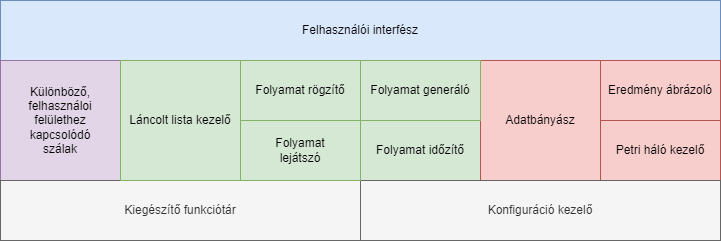
\includegraphics[width=\textwidth,keepaspectratio=true]{images/img_plan_1}
\caption{\textbf{Szerkezeti áttekintő ábra}}
\label{fig:plan}
\end{center}
\end{figure}

\begin{itemize}
	\item \textbf{Felhasználói interfész}: A kezelőfelület, amivel a felhasználó eléri és kezelni tudja az egyes szoftverfunkciókat.
	\item \textbf{Felhasználói felülethez kapcsolódó szálak}: Fontos - a felhasználó számára nem látható - szálak, amelyek feldata bizonyos billentyűkombinációk figyelése anélkül, hogy a program reszponzivitását kártékonyan befolyásolnák.
	\item \textbf{Láncolt lista kezelő}: Az egyes folyamatok láncolt listaként vannak kezelve a szoftverbe, ez az alrendszer felel a megfelelő értelmezésükért. 
	\item \textbf{Folyamat rögzítő}: Figyeli és rögzíti a perifériák általi beviteli értékeket.
	\item \textbf{Folyamat generáló}: Előre meghatározott forgatóvkönyvek alapján úgy generál folyamatokat mintha azt egy felhasználó végezte volna el.
	\item \textbf{Folyamat lejátszó}: A folyamatokat játsza vissza, egy felhasználót szimulál.
	\item \textbf{Folyamat időzítő}: A Windowsba integrált rendszert felhasználva ütemez / időzít folyamatokat.
	\item \textbf{Adatbányász}: Az Alpha-algoritmust implementálva folyamatelemzést hajt végre több folyamaton.
	\item \textbf{Eredmény ábrázoló}: Az Adatbányász által elvégzett folyamatelemzés eredmé\hyp{}nyeit jeleníti meg.
	\item \textbf{Petri-háló kezelő}: A Petri-hálót mint struktúra, valamint a hozzátartozó függ\hyp{}vényeket a szoftver számára értelmezhető módon implementálja.
	\item \textbf{Kiegészítő funkciótár}: Számos hasznos funkció gyűjteménye, melyet a többi alrendsze használ.
	\item \textbf{Konfiguráció kezelő}: Futásidők között felhasználói preferenciák és beállítások tárolásáért és betöltéséért felel.
\end{itemize}

\Section{Folyamatelemzés}

Az Alpha-algoritmust mint folyamatelemzési módszert hasznosan lehet alkalmazni a dolgozati témában. Az algoritmus, jelentőségét tekintve elengedhetetlen részét képezi a dolgozatnak. Jelen esetben a folyamatokat azok jellegétől és céljától függetlenül lehet elemezni, akár cél nélküli beviteli sorozatra is alkalmazható az Alpha-algoritmus.

\subsection{Az Alpha-algoritmus}

Ebben az alfejezetben bemutatásra kerül, hogy hogyan is kapcsolódik pontosan az Alpha-algoritmus a dolgozat témájához.

Először is pontosan meg kell határozni, hogy milyen lépésekből áll az algoritmus.

\begin{definition}{\textit{($\alpha$-algoritmus):}} Legyen $L$ egy eseménynapló adott $E$ események hal\hyp{}maza felett. Ekkor a kimeneti $\alpha (L)$ Petri-hálót az alábbi módon határozzuk meg:
\begin{enumerate}
	\item Definiáljuk az összes eseményt.\\
	\[
		E_L = \{ e \in E | \exists_{\sigma \in L} e \in \sigma \},
	\]
	\item Definiáljuk az összes bemeneti eseményt.
	\[
		E_I = \{ e \in E | \exists_{\sigma \in L} e = first(\sigma) \},
	\]
	\item Definiáljuk az összes kimeneti eseményt.
	\[
		E_O = \{ e \in E | \exists_{\sigma \in L} e = last(\sigma) \},	
	\]
	\item Kiszámítjuk az összes lehetséges $A$ és $B$ halmazt úgy, hogy az összes esemény $A$-ban és $B$-ben függetlenek legyenek egymástól, valamint minden $A$-beli esemény okozati kapcsolatban álljon $B$-beli eseményekhez.
	\begin{equation*}
	\begin{aligned}
		X_L=
		&\{ (A,B) | A \subseteq E_L \land A \neq \emptyset \land B \subseteq E_L \land B \neq \emptyset \land \\
		&\forall_{a \in A} \forall_{b \in B} a \rightarrow_L b \land \forall_{a1,a2 \in A} a_1\#_L a_2  \land \forall_{b1,b2 \in B} b_1\#_Lb_2\},
	\end{aligned}
	\end{equation*}
	\item Elhagyjuk a nem-maxmiális halmazokat.
	\[
		Y_L = \{ (A,B) \in X_L | \forall_{A',B' \in X_L} A \subseteq A' \land B \subseteq B' \Rightarrow (A,B) = (A',B') \},
	\]
	\item Helyeket rendelünk az összes származtatott halmazhoz valamint a kezdő- és végál\hyp{}lapotokhoz.
	\[
		P_L = \{ p_{A,B} | (A,B) \in Y_L\} \cup \{i_L,o_L\},		
	\]
	\item Berajzoljuk a kapcsolatokat.
	\begin{equation*}
	\begin{aligned}
		F_L=
		&\{(a,p_{(A,B)} | (A,B) \in Y_L \land a \in A \} \cup \{ (p_{(A,B)}, b) | (A,B) \in \\
		&Y_L \land b \in B \} \cup \{ (i_L,e) | e \in E_I \} \cup \{ (e,o_L) | e \in E_O\},
	\end{aligned}
	\end{equation*}
	\item Visszatérünk a Petri-hálóval.
	\[
		\alpha(L) = (P_L, E_L, F_L).
	\]

\end{enumerate}

\cite{article:001}
\end{definition}

\begin{example}
	Itt három előre létrehozott folyamaton kerül alkalmazásra az algoritmus. A folyamatok egyszerűek, hogy szemléletes legyen a példa, viszont ugyanezzel a mód\hyp{}szerrel több száz vagy akár több ezer hosszú folyamaton is alkalmazható az algoritmus.
	
	Maguk a folyamatok szolgálnak bemenetként, részeredményekként eseménynapló és lenyomati mátrix jön létre, kimentként pedig egy olyan Petri-háló kerül generálásra mely leírja a folyamat modelljét.

	Vegyük a 3.1. táblázatot.
	\newpage

	\begin{table}[h!]
	\begin{center}
	\caption{Beviteli folyamatok}
	\begin{tabular}{|| c | c | c | c | c | r ||}
		\hline\hline
		\textbf{Folyamat} & \textbf{ID} & \textbf{Típus} & \textbf{Érték} & \textbf{Érték típusa} &  \textbf{Eltelt idő} \\ [0.5ex]
		\hline\hline
		1 & 1 & Key&  Left Alt & WM\_SYSKEYDOWN & 0 \\
		\hline
		1 & 2 & Key&  F4 & WM\_SYSKEYDOWN & 100 \\
		\hline
		1 & 3 & Key&  F4 & WM\_SYSKEYUP & 150 \\
		\hline
		1 & 4 & Key&  Left Alt & WM\_KEYUP & 612 \\
		\hline\hline
		2 & 1 & Key & Left Alt & WM\_SYSKEYDOWN & 0 \\
		\hline
		2 & 2 & Key & F4 & WM\_SYSKEYUP & 80 \\
		\hline
		2 & 3 & Key & F4 & WM\_SYSKEYDOWN & 51 \\
		\hline
		2 & 4 & Key & Left Alt & WM\_KEYUP & 152 \\
		\hline\hline
		3 & 1 & Key & Left Alt & WM\_SYSKEYDOWN & 0 \\
		\hline
		3 & 2 & Mouse & 25:1022 & WM\_LBUTTONDOWN & 151 \\
		\hline
		3 & 3 & Key & Left Alt & WM\_KEYUP & 188 \\
		\hline\hline
	\end{tabular}
	\label{fig:planexample}
	\end{center}
	\end{table}	

	Az Alpha-algoritmus alkalmazásában, mint bármely folyamatbányászati algorit\hyp{}musnál, első lépésként ezekből az eseményekből fel kell építeni az eseménynaplót amiből később dolgozik az algoritmus. Ez a lépés konkrétan arról szól, hogy a már meglévő folyamatok az Alpha-algoritmusnak szükséges formátumra kerülnek átalakításra.
	
	Ez jelen esetben az alábbi három szabály alapján történik:
	\begin{enumerate}
		\item A "\textbf{Folyamat}" elnevezésű oszlop alapján triviális módon meghatározásra kerül az esethez tartozó egyedi azonosító,
		\item A "\textbf{Típus}", "\textbf{Érték}" és "\textbf{Érték típusa}" oszlophármas értékeiből létrejön a tevékenység megnevezése,  ami a továbbiakban \textit{,,$T_{n}$"}-ként lesz feltüntet\hyp{}ve,
		\item Az "\textbf{Eltelt idő}" oszlop alapján (az előző esemény óta eltelt időt mutatja) pedig létrejön egy relatív-időbélyeg az "\textbf{ID}" oszlop segítségével, hiszen az utóbbi alap\hyp{}ján határozható meg az események szekvenciája.
	\end{enumerate}
	
	Ezeknek megfelelően a 3.2. táblázatban látható eseménynaplót kapjuk.
	\newpage

	\begin{table}[h]
	\begin{center}
	\caption{Eseménynapló}
	\begin{tabular}{|| c | c | c ||}
		\hline
		Azonosító & Tevékenység & Relatív időbélyeg \\ [0.5ex]
		\hline\hline
		1 & $T_0$ & 0 \\
		\hline
		1 & $T_1$ & 100 \\
		\hline
		1 & $T_2$ & 250 \\
		\hline
		1 & $T_3$ & 762 \\
		\hline
		2 & $T_0$ & 0 \\
		\hline
		2 & $T_2$ & 80 \\
		\hline
		2 & $T_1$ & 131 \\
		\hline
		2 & $T_3$ & 283 \\
		\hline
		3 & $T_0$ & 0 \\
		\hline
		3 & $T_4$ & 151 \\
		\hline
		3 & $T_3$ & 339 \\
		\hline
	\end{tabular}
	\label{fig:planexample}
	\end{center}
	\end{table}	
	
	Miután megvan az eseménynapló, a következő két lépésben meghatározzuk a beme\hyp{}neti- és kimeneti események halmazait:
	\begin{enumerate}
		\item $E_I=<T_0>$,
		\item $E_O=<T_3>$.
	\end{enumerate}

	Ezután a következő lépéshez az eseménynaplóban szereplő események kapcsolatait közvetlen-sorrend, okozat, párhuzam és választás relációkra alakítja az algoritmus.

	Ezzel jön létre a 3.3. táblázatban látható lenyomati mátrix.
	
	\begin{table}[h]
	\begin{center}
	\caption{Lenyomati mátrix}
	\begin{tabular}{|c | c | c | c | c | c|}
		\hline
		\hspace{0.1cm} & $T_0$ & $T_1$ & $T_2$ & $T_3$ & $T_4$ \\
		\hline
		$T_0$ & \# & $\rightarrow$ & $\rightarrow$ & \# & $\rightarrow$ \\
		\hline
		$T_1$ & $\leftarrow$ & \# & $\parallel$ & $\rightarrow$ & \# \\
		\hline
		$T_2$ & $\leftarrow$ & $\parallel$ & \# & $\rightarrow$ & \# \\
		\hline
		$T_3$ & \# & $\leftarrow$ & $\leftarrow$ & \# & $\leftarrow$ \\
		\hline
		$T_4$ & $\leftarrow$ & \# & \# & $\rightarrow$ & \# \\
		\hline
	\end{tabular}
	\label{fig:planexample}
	\end{center}
	\end{table}

	Ezen a mátrixon kerül ábrázolásra az összes esemény közötti kapcsolat. Több szem\hyp{}pontból is hasznos ez a mátrix, többek között a struktúrája is megfelelő ahhoz, hogy program szinten meghatározzuk a következő lépésben a lehetséges halmazpárokat, vala\hyp{}mint emberi szemmel is kifejezetten könnyen értelmezhető.

	Ezt a mátrixot felhasználva a 3.4. táblázatban látható halmazpárok lehetségesek a jelenlegi példában:
	\newpage

	\begin{table}[h]
	\begin{center}
	\caption{Lehetséges halmazpárok}
	\begin{tabular}{|| c | c ||}
		\hline
		A & B \\
		\hline\hline
		\{$T_0$\} & \{$T_1$\} \\
		\hline
		\{$T_0$\} & \{$T_2$\} \\
		\hline
		\{$T_0$\} & \{$T_4$\} \\
		\hline
		\{$T_1$\} & \{$T_3$\} \\
		\hline
		\{$T_2$\} & \{$T_3$\} \\
		\hline
		\{$T_4$\} & \{$T_3$\} \\
		\hline
		\{$T_0$\} & \{$T_1, T_4$\} \\
		\hline
		\{$T_0$\} & \{$T_2, T_4$\} \\
		\hline
		\{$T_1, T_4$\} & \{$T_3$\} \\
		\hline
		\{$T_2, T_4$\} & \{$T_3$\} \\
		\hline
	\end{tabular}
	\label{fig:planexample}
	\end{center}
	\end{table}	

	Következő lépésként ezekből a halmazpárokból kell eltávolítani a nem-maximálisak\hyp{}at, azaz azokat amik részhalmazai egy másiknak. Ezt program szinten egy többszörös ciklus segítségével könnyedén el lehet végezni, jelen példában pedig az 3.5. táblázatban található, négy halmazpár maradt:
	
	\begin{table}[h]
	\begin{center}
	\caption{Maradék halmazpárok}
	\begin{tabular}{|| c | c ||}
		\hline
		A & B \\
		\hline\hline
		\{$T_0$\} & \{$T_1, T_4$\} \\
		\hline
		\{$T_0$\} & \{$T_2, T_4$\} \\
		\hline
		\{$T_1, T_4$\} & \{$T_3$\} \\
		\hline
		\{$T_2, T_4$\} & \{$T_3$\} \\
		\hline
	\end{tabular}
	\label{fig:planexample}
	\end{center}
	\end{table}

	Miután ezek a halmazpárok meghatározásra kerültek, helyek $(p_1-p_4)$  lesznek hozzájuk rendelve. Ezekhez a helyekhez létrehozásra kerülnek a megfelelő bemeneti és kimeneti átmenetek, valamint a végső bemeneti és kimeneti állapotok is.

	Amint ez megvan, berajzolásra kerülnek a kapcsolatok is, a végén pedig a következő Petri-háló kerül megjelenítésre.\cite{procmining}
	\newpage

	\begin{figure}[h!]
	\begin{center}
	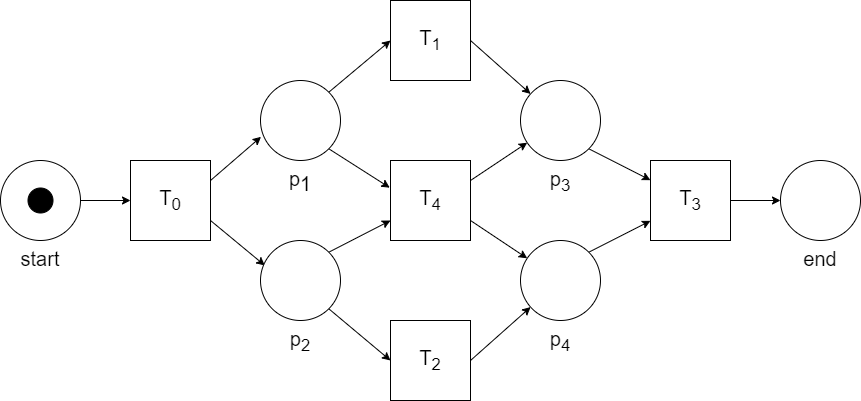
\includegraphics[width=\textwidth,keepaspectratio=true]{images/img_plan_2}
	\caption{Kimeneti Petri-háló}
	\label{fig:plan}
	\end{center}
	\end{figure}

\end{example}


\definecolor{codeComment}{RGB}{0, 128, 0}
\definecolor{codeKeyword}{RGB}{0, 0, 255}
\definecolor{codeNumber}{RGB}{100, 100, 255}
\definecolor{codeString}{RGB}{100, 100, 255}
\lstdefinestyle{delphicode}{
	language=Delphi, 
	commentstyle=\color{codeComment},
	keywordstyle=\color{codeKeyword},
	numberstyle=\tiny\color{codeNumber},
	stringstyle=\color{codeString},
	basicstyle=\ttfamily\footnotesize,
	breaklines=true,
	showspaces=false,
	showstringspaces=false
}
\lstset{style=delphicode}


\Section{Implementáció}

A program gyakorlati megvalósítása egy-két apróságtól eltekintve megegyezik a terve\hyp{}zettel. Fejlesztés közben felmerültek ötletek, melyek javítottak az eredeti terven, de az alapvető stuktúra megmaradt, az egymáshoz tartozó funkciók, változók és kódrészletek pedig külön egységekbe (továbbiakban: unitok) lettek szervezve, így csoportosítva az egyes szoftverfunkciókat.

Ezek a unitok többféle kapcsolatban állhatnak egymással, az egymásra való hivatko\hyp{}zásuknak függvényében. Ezeket a kapcsolatokat a 3.3 ábra demonstrálja.

\begin{figure}[h]
	\begin{center}
		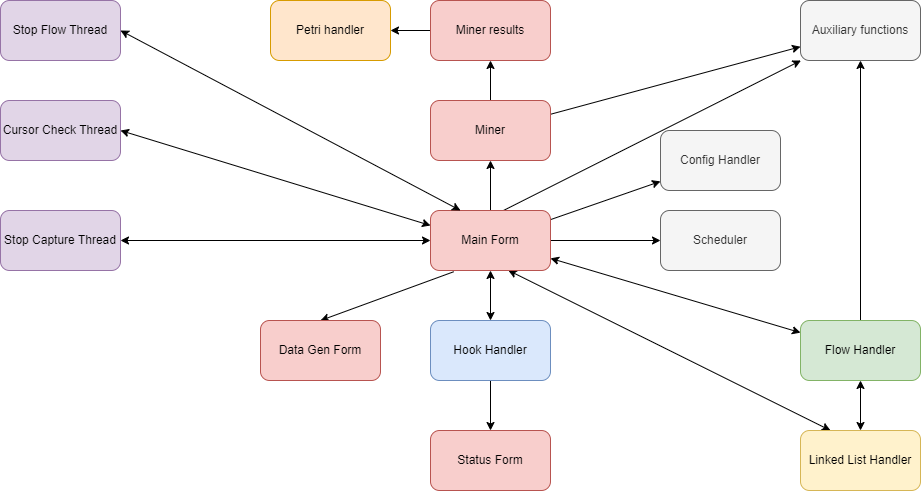
\includegraphics[width=0.95\textwidth, keepaspectratio=true]{images/unitok_kapcsolati_abra}\\
		\label{fig:example}
	\end{center}
	\caption{Unitok kapcsolatai}
\end{figure}

Pirossal azok a unitok láthatók melyekhez tartozik grafikus felület is, a további színek pedig az egyes funkciók csoportosítására szolgálnak. Részletesebben a unitokról a következő pontokban olvashatunk.

\begin{itemize}
	\item{
		\textbf{Unit\_Main}: Ez a program főegysége, ebben került implementálásra a főablak és annak felhasználói felülete. Az alábbi feladatokat látja el.
		\begin{enumerate}
			\item{Implementálja a felhasználói felület objektumait, azoknak a tulajdonságait és rutinjait.}
			\item{Inicializálja a programot futtatásnál, betölti a felhasználó konfigurációit.}
			\item{Kezeli a program rendszertálcára való kicsinyítését.}
			\item{Kezeli azt a néhány globális változót amik szükségesek (pl.: a futtatható fájl elérési útvonala).}			
		\end{enumerate}
	}
	\item{
		\textbf{Unit\_ConfigHandler}: A konfigurációkezelő osztályt, az abba tartozó objek\hyp{}tumokat és rutinokat implementálja, melyek lehetővé teszik a futásidő alatti konfigurációs beállítások titkosítva történő tárolását.
		\begin{lstlisting}
  TConfigHandler = class(TObject)
    configFile: string;
    configArray: array of array of string;

  public
    procedure Save(Key: string; Value: string);
    function Load(Key: string; Fallback: string): string;

    constructor Create(filePath: string);
    destructor Destroy; override;

    function Encrypt(const value: string): UnicodeString;
    function Decrypt(const value: string): UnicodeString;

    function MatchCharToArrayIndex(const character: char): integer;
  end;
		\end{lstlisting}
	}
	\item{
		\textbf{Unit\_AuxiliaryFunctions}: Néhány olyan kiegészítő rutint tartalmazó gyűjte\hyp{}mény, melyeket a többi egység használ. Külön egységbe ki lettek gyűjtve, hogy az OOP alapelvek teljesüljenek.
	}
	\item{
		\textbf{Unit\_StopFlowThread}: Egy olyan szálat implementáló egység, amely feladata kifejezetten a \textbf{F2 + F3} billentyűkombináció lenyomásának felügyelete.

		Ez a billentyűkombináció felel azért, hogy az éppen futó folyamatot le lehessen futás közben állítani. Feltétlenül szükséges, hogy ez ilyen módon legyen implemen\hyp{}tálva, hiszen ennek a billentyűkombinációnak akkor is működnie kell, ha a fókusz éppen egy másik alkalmazáson van.

A Windows API és a \textbf{Unit\_Main} által implementált rutinokra és változókra hivatkozik a műküdése során.
		\begin{lstlisting}
procedure TStopFlowThread.Execute;
begin
  repeat
    if (GetKeyState(VK_F2) < 0) and (GetKeyState(VK_F3) < 0) then
    begin
      Form1.Btn_StartFlowClick(stopFlowThread);
    end;
  until not runStopFlow;
end;
		\end{lstlisting}
	}
	\item{
		\textbf{Unit\_CursorCheckThread}: Egy olyan szálat implementáló egység, melynek feladata a kurzor aktuális pozíciójának a felhasználói felületen történő frissítése. Windows API-t meghívva jut hozzá a szükséges adathoz.
		\begin{lstlisting}
procedure TCursorCheckThread.Execute;
var
  p: TPoint;
begin
  FreeOnTerminate := true;
  repeat
    GetCursorPos(p);
    Form1.Lab_Cursor_X.Caption := 'x: ' + IntToStr(p.X);
    Form1.Lab_Cursor_Y.Caption := 'y: ' + IntToStr(p.Y);
  until not runCursorPos;
end;
		\end{lstlisting}
		Ennek a célja, az, hogy amikor a felhasználó kézileg akar egérkattintást hozzáadni az aktuális folyamathoz, akkor megkönnyítse a megfelelő képernyő-koordináták meghatározását.
	}
	\item{
		\textbf{Unit\_StopCaptureThread}: Egy olyan szálat implementáló egység, melynek feladata hasonló az előzőekben bemutatott \textbf{TStopFlowThread}-éhez.

Az eltérés annyi, hogy az \textbf{F2 + F4} billentyűkombinációt figyeli, melynek lenyo\hyp{}mására egy olyan rutint hív meg, mely leállítja az éppen futó felhasználói ese\hyp{}ménysor rögzítését.
	}
	\item{
		\textbf{Unit\_LinkedListHandler}: Egy olyan struktúrát implementál, melyre a szoft\hyp{}ver összes többi folyamatkezezlő egysége épül. Az ebből a láncolt lista struktúrá\hyp{}ból példányosított elemek tartalmazzák a folyamat lépéseihez tartozó összes infor\hyp{}mációt.

	Először is implementál két felsorolás típust, melyek intuitív módon leírják magu\hyp{}kat:
	\begin{lstlisting}
type
  // Enum
  TInputType = (itClick, itKeyboard, itSpecialKey, itHotkey);
  TWaitType = (wtMil, wtSec, wtMin, wtHour);
	\end{lstlisting}

	valamint definiálja a láncolt lista elemet és az arra hivatkozó mutatót:
	\begin{lstlisting}
  // Linked List pointer type
  PFlowElement = ^TFlowElement;

  // Linked List element
  TFlowElement = record
    inputType: TInputType;
    inputParam1: string;
    inputParam2: string;
    inputParam3: string;
    inputParam4: string;
    waitAfterAmount: integer;
    waitAfterType: TWaitType;
    waitAfterTypeText: string;
    deleteButton: TButton;
    panelObject: TPanel;
    labelObject: TLabel;
    NextElement: PFlowElement;
  end;
	\end{lstlisting}

	Ezek mellett még tartalmaz egy rutint, mely arra szolgál, hogy egy meglévő láncolt lista elemtől kezdve az összes további elemhez tartozó objektumot megfele\hyp{}lően szabadítsa fel a memóriából.

	}
	\item{
		\textbf{Unit\_FlowHandler}: A folyamatokhoz tartozó legfontosabb rutinokat definiál\hyp{}ja, amik a következőek:
		\begin{enumerate}
			\item{folyamat mentése fájlba,}
			\item{folyamat betöltése állományból,}
			\item{folyamat generálása a felhasználói bevitelből rögzített eseméysorból,}
			\item{adott folyamati lépés végrehajtása, azaz input injektálása a Windows felé. pl.:
				\begin{lstlisting}
if (currentStep.inputParam3 = 'Left') and
(currentStep.inputParam4 = 'Down+Up (single)') then
begin
  mouse_event(MOUSEEVENTF_LEFTDOWN, 0, 0, 0, 0);
  mouse_event(MOUSEEVENTF_LEFTUP, 0, 0, 0, 0);
end 
				\end{lstlisting}
			} 
			
		\end{enumerate}
	}
	\item{
		\textbf{Unit\_HookHandler}: Ennek az egységnek a feladata azoknak az objektumok\hyp{}nak, változóknak és függvényeknek az implementációja, melyek lehetővé teszik a felhasználói input rögzítését a Windows API \textit{hook}-jainak felhasználásával.

A \textit{hook} egy olyan pont a rendszer üzenetkezelő mechanizmusában, ahová a szoft\hyp{}ver egy olyan szubrutint telepít, mely figyeli az üzenet forgalmat a rendszerben, és feldolgozza azokat még mielőtt elérné a cél-ablakhoz tartozó eljárását.

A felhasználói input rözítésénél két ilyen \textit{hook} kerül telepítésre: egy a billentyűzet üzenetsornak, a másik pedig az egérhez tartozóhoz. Ezek a telepítések a Win\hyp{}dows API által biztosított
\begin{lstlisting}
function SetWindowsHookEx; external user32 name 'SetWindowsHookExW';
\end{lstlisting}
függvény hívásával történnek.

Ezeken túl az egység tartalmaz egy olyan funkciót is, mely az adott konstanst (vagy karakterkódot) ember által könnyen értelmezhető szövegre fordítja, pl. \textbf{VK\_PRIOR} $\rightarrow$ \textbf{[Page Up]}, vagy \textbf{65} $\rightarrow$ \textbf{[a]}

	}
	\item{
		\textbf{Unit\_Status}: Ez az egység azt az ablakot implementálja, mely visszajelzést ad az éppen futó eseménysor-rögzítés lépéseiről.
		\begin{lstlisting}
type
  TForm_Status = class(TForm)
    Lab_Input: TLabel;
    Lab_Finish: TLabel;
    Lab_Input_Title: TLabel;
    Lab_StepID_Title: TLabel;
    Pnl_Main: TPanel;
    Lab_StepID: TLabel;
    procedure FormCreate(Sender: TObject);
    procedure FormShow(Sender: TObject);
    procedure FormMouseMove(Sender: TObject; Shift: TShiftState; X, Y: Integer);
  public
    procedure UpdateLabel_Input(newText: string);
    procedure UpdateLabel_StepID(newID: integer);
  end;
		\end{lstlisting}

A rutinjai lehetővé teszik, hogy más egységből (pl.:\textbf{Unit\_HookHandler}) is lehes\hyp{}sen frissíteni a grafikus elemeit, valamint, hogy folyamatrögzítés közben hiába látszik az ablak, akkor se legyen útban a felhasználónak.
	}
	\item{
		\textbf{Unit\_Scheduler}: Két egyszerű függvényt implementáló osztályt definiál, mely arra szolgál, hogy a Windows API segítségével meghívott \textit{schtasks.exe} feladatüte\hyp{}mezőbe rögzíteni, illetve onnan törölni lehessen folyamatokat.
	\begin{lstlisting}
  TScheduleHandler = class(TObject)
  public
    function DeleteTask(fPath: string): integer;
    function AddTask(fPath, sPath: string): integer;
  end;
	\end{lstlisting}
	}
	\item{
		\textbf{Unit\_DataGenerator}: Egy felületet és számos rutint definiál, melyek segítsé\hyp{}gével könnyedén folyamatokat lehet generálni. Ennek az a célja, hogy az adatbá\hyp{}nyászathoz elegendő mennyiségű folyamatot lehessen meghatározni emberi időn belül.

	\begin{lstlisting}
type
  TForm_Generator = class(TForm)
    Mem_Log: TMemo;
    Pnl_Interface: TPanel;
    Btn_Generate: TButton;
    RadGroup_GenCategory: TRadioGroup;
    Spin_GenCount: TSpinEdit;
    procedure Btn_GenerateClick(Sender: TObject);
    procedure FormCloseQuery(Sender: TObject;
    var CanClose: Boolean);
  private
    { Private declarations }
    procedure Generate_ComputerShutdown(count: integer);
    procedure Generate_ComputerRestart(count: integer);
    procedure Generate_BrowserLaunch(count: integer);
    procedure AddToLog(msg: string);

    function GetClickDelay(_type: integer): integer;
    function GetRandomMouseCoordinate(min, max: integer):integer;
  end;

	\end{lstlisting}

		Három forgatókönyv került létrehozásra, ezekből választva lehetséges a generálás. A feladatot elvégezve a folyamatokat egy adott mappába állományonként menti le a szoftver.
	}
	\item{
		\textbf{Unit\_Miner}: Egy felület ami az Alpha-algoritmust illetve a Heurisztikus Bá\hyp{}nyászt  implementálja. A felületet használva a bányászat megkezdését követően láthatjuk, hogy éppen hol jár a választott algoritmustban a szoftver.
	\begin{lstlisting}
type
  TForm_Miner = class(TForm)
    Panel_Interface: TPanel;
    Mem_Log: TMemo;
    Edt_DataPath: TEdit;
    Pnl_DataPath: TPanel;
    Lab_DataPath: TLabel;
    Btn_DataPath_Browse: TButton;
    Btn_Begin: TButton;
    procedure FormCloseQuery(Sender: TObject;
    var CanClose: Boolean);
    procedure Btn_DataPath_BrowseClick(Sender: TObject);
    procedure Btn_BeginClick(Sender: TObject);
  private
    procedure AddToLog(msg: string);
    procedure AlphaMine();
    procedure ChangeUserControl(newState: boolean);
    function RemoveBracketsFromString(str: string): string;
    function IsInActivityList(str: string): boolean;
    function GetNewActivityID: string;
    function FindActivityID(str: string): string;
  end;
	\end{lstlisting}

Amint végzett az algoritmus, az eredményeket a következő \textbf{Unit\_MinerResults} által definiált ablakban ábrázolja.

A halmazpárok három-dimenziós adatstruktúrában vannak tárolva, illetve kezel\hyp{}ve. Ezeknek az értelmezése elég komoly odafigyelést igényel.
	\begin{lstlisting}
  TArrayOfSets = array of array of array of integer;
	\end{lstlisting}

	}
	\item{
		\textbf{Unit\_MinerResults}: Azt a felületet implementáló egység, mely a választott bányász eredményeit jeleníti meg grafikusan. Ezek:
		\begin{enumerate}
			\item{a létrejött eseménynapló,}
			\item{az eseménynaplóbó létrejött lenyomati mátrix (Heurisztikus bányásznál füg\hyp{}gőségi mátrix),}
			\item{az összes maximális halmaz (Alpha-algoritmus esetében),}
			\item{a kimeneti Petri-háló, melyet a \textbf{Unit\_PetriHandler} segítségével generál.}
		\end{enumerate}
		\begin{lstlisting}
  TForm_MinerResults = class(TForm)
  .
  .
  .
  public
    procedure DrawPetriNet(arrayOfSets: TArrayOfSets);
    procedure DrawPlace(startX, startY: integer; lab: string);
    procedure DrawTransition(startX, startY: integer; lab: string);

    procedure DrawArrow(startX, startY, endX, endY: integer); overload;
    procedure DrawArrow(endX, endY: integer); overload;

    function GetStartEvents(): TIntegerArray;
    function GetEndEvents(): TIntegerArray;
  end;

		\end{lstlisting}
	}
	\item{
		\textbf{Unit\_PetriHandler}: Számos objektumot és rutint implementál, melyek segít\hyp{}ségével felépíthető és megjeleníthető egy Petri-háló.
		\begin{enumerate}
			\item{Definiálja a helyeket,
				\begin{lstlisting}
  TPetriPlace = record
    name: string;
    fromList: TStringArray;
    toList: TStringArray;
    location: TPoint;
    recursionLock: boolean;
  end;
				\end{lstlisting}
			}
			\item{Definiálja az átmeneteket,
				\begin{lstlisting}
  TPetriTransition = record
    id: integer;
    fromList: TStringArray;
    toList: TStringArray;
    location: TPoint;
    recursionLock: boolean;
  end;
				\end{lstlisting}
			}
			\item{Definiál egy Petri-háló gyűjteményt, melyben tárolni lehet a helyeket és átmeneteket, valamint a rutinok segítségével fel lehet térképezni a közöttük lévő kapcsolatokat.
				\begin{lstlisting}
  TPetriCollection = class(TObject)
    places: array of TPetriPlace;
    transitions: array of TPetriTransition;
    objectSize: integer;
  public
    constructor Create();
    destructor Destroy(); override;
    procedure NewPlace(_name: string; _fromList, _toList: TStringArray);
    procedure NewTransition(_id: integer; _fromList, _toList: TStringArray);
    function FindIndexOfPlace(name: string): integer;
    function FindIndexOfTransition(id: integer): integer;
    procedure MapTransitions();
    procedure MapPlaceLocation(currentTransition: TPetriTransition);
    procedure MapTransitionLocation(currentPlace: TPetriPlace);
    procedure UpdateList(var list: TStringArray; newValue: string);
    function GetMaxIndexInColumn(col: integer): integer;
  end;
				\end{lstlisting}
 Indexek alapján kerülnek meghatározásra a helyek és átmenetek közötti kapcsolatok, így a megjelenített ábra balról-jobbra értelmezendő.
			}
		\end{enumerate}
	}
\end{itemize}























